\appendix

\chapter{Kristalografske oznake i grupe}
\label{sec:kristalografija}
\textbf{Ireducibilne reprezentacije} $\Gamma^{(\alpha)}$ se obično označavaju
velikim slovima i to tako da se 1D reprezentacije označavaju slovima
$A$ i $B$, 2D reprezentacije slovom $E$, 3D reprezentacije slovom $T$
itd. Par kompleksno konjugiranih 1D reprezentacija se smatra jednom
2D reprezentacijom (jer ih povezuje vremenska inverzija) tako da se
one udružuju vitičastom zagradom i označavaju s $E$.

\textbf{Klase konjugacije} se obično označavaju simbolom $mC_n$ gdje je $m$
broj elemenata klase, a $C_n$ tipični predstavnik klase označen
Sch\"{o}nfliesovim simbolom:
\begin{center}
\begin{tabular}{rcp{10cm}}
$E$ & = & identiteta \\
$C_n$ & = & rotacija za $2\pi/n$ \\
$\sigma$ & = & refleksija preko ravnine \\
$\sigma_{h}$ & = & refleksija preko ``horizontalne'' ravnine tj. ravnine
  okomite na os najveće rotacijske simetrije \\
$\sigma_{v}$ & = & refleksija preko ``vertikalne'' ravnine tj. ravnine
  koja sadrži os najveće rotacijske simetrije \\
$\sigma_{d}$ & = & refleksija preko ``dijagonalne'' ravnine tj. ravnine
  koja sadrži os najveće rotacijske simetrije i raspolavlja kut između
  dvije $C_2$ osi okomite na tu os. (Specijalni slučaj $\sigma_{v}$.) \\
$S_n$  & = & rotacija za $2\pi/n$ kombinirana s refleksijom preko ravnine
   okomite na os te rotacije (Ove dvije operacije komutiraju.) \\
$i$ & = &  $S_2 \;\, = \;\,$  inverzija $\vec{r} \to -\vec{r}$
\end{tabular}
\end{center}
Ako ima više istovrsnih klasa, označavamo ih po redu npr.
$C_{2}$, $C_{2}'$, $C_{2}''$, itd.

\textbf{Točkaste grupe} kristala se označavaju slijedećim
Sch\"{o}nfliesovim oznakama:
\begin{center}
\begin{tabular}{rcl}
$C_n$ & = & grupe s jednom $C_n$ osi simetrije \\
$C_{nv}$ & = & grupe s jednom $C_n$ osi i $n$ $\sigma_v$
   refleksijskih ravnina  \\
$C_{nh}$ & = & $C_n$ os,  $\sigma_h$ refleksija $+$ dodaci \\
$S_{n}$ & = & $S_n$ os \\
$D_{n}$ & = & $C_n$ os i $n$ $C_2$ osi okomitih na nju \\
$D_{nd}$ & = & elementi od $D_{n}$ i $\sigma_d$ ravnine refleksije \\
$D_{nh}$ & = & elementi od $D_{n}$ i $\sigma_h$ ravnina refleksije \\
$T$  & = & tetrahedralna grupa \\
$O$  & = & oktahedralna grupa 
\end{tabular}
\end{center}

\textbf{Tablice karaktera} nekih grupa koje se pojavljuju u ovoj knjizi

Ciklička grupa C$_3$:
\begin{center}
\begin{tabular}{c|ccc}
     & $E$ & $C_3$ & $C_{3}^2$ \\ \hline
    $A$ & 1 & 1 & 1 \\
    \multirow{2}{*}{$E$} & 1 & $\omega$ & $\omega^2$ \\
     & 1 & $\omega^2$ & $\omega$ \\
\end{tabular}
\end{center}
gdje je $\omega = e^{2\pi i/3}$ kubni korijen jedinice i
gdje su zadnje dvije ireducibilne reprezentacija međusobno
kompleksno konjugirane pa se često smatraju jednom dvodimenzionalnom
reprezentacijom $E$.

Ciklička grupa C$_4$:
\begin{center}
\begin{tabular}{c|cccc}
     & $E$ & $C_4$ & $C_2$ & $C_{4}^3$ \\ \hline
    $A$ & 1 & 1 & 1 & 1 \\
    $B$ & 1 & -1 & 1 & -1 \\
    \multirow{2}{*}{$E$} & 1 & $i$ & -1 & $-i$ \\
     & 1 & $-i$ & -1 & $i$ \\
\end{tabular}
\end{center}

Kleinova četvorna grupa D$_2$
\begin{center}
\begin{tabular}{c|cccc}
     & $E$ & $C_{2}(z)$ & $C_{2}(y)$ & $C_{2}(x)$ \\ \hline
    $A_1$ & 1 & 1 & 1 & 1 \\
    $B_1$ & 1 & 1 & -1 & -1 \\
    $B_2$ & 1 & -1 & 1 & -1 \\
    $B_3$ & 1 & -1 & -1 & 1 \\
\end{tabular}
\end{center}

Dihedralna grupa D$_3$
\begin{center}
\begin{tabular}{c|ccc}
  & E & 2$C_3$  & 3$C_2$ \\ \hline
$A_1$ & 1 & 1& 1 \\
$A_2$ & 1 & 1&-1 \\
 $E$  & 2 &-1& 0
\end{tabular}
\end{center}


Dihedralna grupa D$_{4}$
\begin{center}
    \begin{tabular}{c|ccccc}
         & $E$ & $2C_4$ & $C_2$ & $2C_{2}'$ & $2C_{2}''$ \\ \hline
        $A_1$ & 1 & 1 & 1 & 1 & 1 \\
        $A_2$ & 1 & 1 & 1 & -1 & -1 \\
        $B_1$ & 1 & -1 & 1 & 1 & -1 \\
        $B_2$ & 1 & -1 & 1 & -1 & 1 \\
        $E$ & 2 & 0 & -2 & 0 & 0 \\
    \end{tabular}
\end{center}
Ova je grupa izomorfna grupi C$_{4v}$, samo što su u tom  slučaju
neke rotacije za $\pi$ zapravo refleksije: $C_{2}' \to \sigma_v$ i
$C_{2}'' \to \sigma_h$.


Tetrahedralna grupa T:

\begin{center}
\begin{tabular}{c|cccccccc}
 & $E$ & $3C_2$ & $4C_3$ & $4C_{3}^2$  \\ \hline
$A$ & 1 & 1 & 1 & 1  \\
\multirow{2}{*}{$E$} & 1 & 1 & $\omega$ & $\omega^2$ \\
 & 1 & 1 & $\omega^2$ & $\omega$  \\
$T$ & 3 & -1 & 0 & 0  \\
\end{tabular}
\end{center}
gdje je $\omega = e^{2\pi i/3}$ kubni korijen jedinice.



\chapter{Aksijalni vektori (pseudovektori)}
\label{sec:aksijalni}

\emph{Aksijalni} ili \emph{pseudovektori} su objekti koji se pri rotacijama transformiraju
isto kao i obični (tzv. \emph{polarni}) vektori, ali pri refleksijama i inverzijama
imaju još i dodatnu promjenu predznaka.

Inverzija običnim vektorima u 3D euklidskom prostoru mijenja
predznak 
$$i: \vec{r} \to - \vec{r}$$ 
i može se reprezentirati dijagonalnom
matricom 
$$
i = -\Eins = 
\begin{pmatrix}
    -1 & 0 & 0 \\
    0 & -1 & 0 \\
    0 & 0 & -1
\end{pmatrix} \;.
$$
No, vektorski produkt dvaju polarnih vektora, npr. vektora položaja $\vec{r}$
i impulsa $\vec{p}$ posljedično \emph{ne mijenja} predznak:

\[  \vec{L}\equiv \vec{r}\times\vec{p} \; \stackrel{i}{\longrightarrow} \;
  (-\vec{r}) \times (-\vec{p}) =  \vec{r}\times\vec{p} = \vec{L}  \;,
\]

što znači da je $\vec{L}$ (moment impulsa) aksijalni vektor. (U fizici su
veličine vezane uz vrtnju, poput momenta impulsa ili momenta sile, 
često reprezentirane aksijalnim vektorima. Isto vrijedi za veličine
vezane uz magnetizam koji je obično rezultat kruženja (mikro ili makro) struja.)

Da bi se naglasila njihova različitost,
ponegdje u literaturi se aksijalne vektore ne crta kao usmjerene crte
(strelice), već kao crte s ``aksijalnim strelicama'' (cf. 
\cite{Bronstejn:2004} p. 186)

\centerline{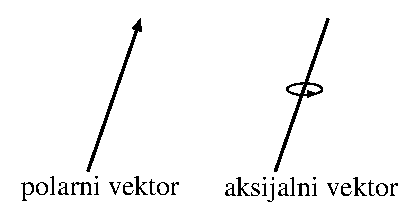
\includegraphics[scale=0.8]{pics/aksijalni_vektor.eps}}

Slično definiramo \emph{pseudoskalarne} veličine kao one koje su skalari
obzirom na rotacije, ali mijenjaju predznak pri refleksijama i inverzijama.
Npr. miješani produkt polarnih vektora je pseudoskalar:

\[
P = (\vec{r}_1 \times \vec{p}) \cdot \vec{r}_2  \; \stackrel{i}{\longrightarrow} \;
  - (\vec{r}_1 \times \vec{p}) \cdot \vec{r}_2 = - P
\]

Magnetski moment, definiran kao $\vec{M} = \frac{1}{2} \int \vec{r}
\times \vec{J} dV$ za gustoću struje $J$, odnosno kao
$\vec{M} = \frac{1}{2} q \vec{r} \times \vec{v}$ za točkasti
naboj $q$, je dakle aksijalni vektor.

Za još o pseudovektorima i drugim pseudo-veličinama vidi
npr. \cite{Arfken:1995}.


\chapter{Kvantna mehanika u Diracovoj notaciji}
\label{sec:qm}

\textbf{Fizikalno stanje} kvantnomehaničkog sustava
je reprezentirano vektorom u Hilbertovom prostoru za
koji se koristi Diracova oznaka
 $\ket{\alpha}$ --- tzv. "ket". 
(Strogo uzevši, kvantnom stanju odgovara
čitava "zraka" $c\ket{\alpha}, c\in\mathbb{C}$.)

Simbol $\alpha$ ovdje stoji za sve kvantne brojeve koji su potrebni za potpuno
određenje stanja. Npr, za vodikov atom $\ket{\alpha}=\ket{n,l,m}$.
Svakom vektoru odgovara dualni "bra" vektor $\bra{\alpha}$, tako
da skalarni produkt zapisujemo kao "bra-ket"A
$\bra{\alpha}\beta \rangle$. Kako je riječ o vektorskom prostoru
nad kompleksnim poljem, vrijedi
$\bra{\alpha}\beta \rangle^{*} = \bra{\beta}\alpha \rangle$.

\textbf{Opservabla} (veličina koja se eksperimentalno određuje i ima
 analogon u klasičnoj fizici) je reprezentirana hermitskim operatorom na
 Hilbertovom prostoru prostoru stanja: $A=A^{\dagger}$.

Ako su $\ket{a}$ svojstveni vektori od $A$ sa svojstvenim vrijednostima
$a$, tj.
\begin{displaymath}
                A\ket{a}=a\ket{a} \;,
\end{displaymath}
onda mjerenje klasične veličine koja odgovara operatoru A, na sustavu
opisanom vektorom $\ket{\alpha}$, s vjerojatnošću $|\bra{a}\alpha\rangle|^2$
ima ishod $a$, nakon čega sustav "skače" u stanje $\ket{a}$.

Očekivana vrijednost mjerenja veličine koja odgovara
operatoru $A$, na sustavu opisanom vektorom stanja
$\ket{\alpha}$ je $\bra{\alpha}A\ket{\alpha}$.

Svi svojstveni vektori nekog hermitskog operatora čine jednu bazu
Hilbertovog prostora:
\begin{displaymath}
             \sum_{a} \ket{a}\bra{a} = 1 \,.
\end{displaymath}
Npr. svi vektori $\ket{\vec{r}}$ čine jednu tzv. koordinatnu bazu.
Schr\"{o}dingerova valna funkcija $\psi_{\alpha}(\vec{r})$ su zapravo
komponente vektora stanja $\ket{\alpha}$ prikazane u koordinatnoj
bazi:
\begin{displaymath}
            \psi_{\alpha}(\vec{r})=\bra{\vec{r}}\alpha\rangle
\end{displaymath}


\textbf{Operatori transformacije} fizikalnog sustava (tj. odgovarajućeg vektora
stanja) moraju biti unitarni i linearni (ili antiunitarni i antilinearni)
\begin{align*}
\text{\sl unitarnost}&:\; \bra{U\alpha}U\beta\rangle = \bra{\alpha}\beta\rangle
   \\
\text{\sl linearnost}&:\; U\big(c_1\ket{\alpha}+c_{2}\ket{\beta}\big)=
  c_1 U\ket{\alpha} + c_{2} U\ket{\beta}
   \\[2ex]
\text{\sl antiunitarnost}&:\; \bra{U\alpha}U\beta\rangle = \bra{\alpha}\beta\rangle^*
  \\
\text{\sl antilinearnost}&:\; U\big(c_1\ket{\alpha}+c_{2}\ket{\beta}\big)=
  c_{1}^* U\ket{\alpha} + c_{2}^* U\ket{\beta}
\end{align*}
Ovo je sadržaj tzv. Wignerovog teorema, a u osnovi
je posljedica zahtjeva za očuvanjem vjerojatnosti i
načela superpozicije u kvantnoj mehanici.

